\scanpage{63}
dont la subdivision barycentrique, donnée par
\[
\text{(22)}\qquad
\left\{\begin{aligned}
&S_1=\{1\},\quad S_\infty=\{\infty\},\quad K=\mathbb P^1(\mathbb R)=K_0\cup K_1\cup K_\infty\\
&\text{avec}\qquad K_0=[1,\infty],\quad K_1^{\unsure{\prime|!}}=[\infty,0],\quad
\underbrace{K_\infty=[0,1]}_{\substack{\text{comme avant}\\\text{cf (21)}}}
\end{aligned}\right.
\]
\figure{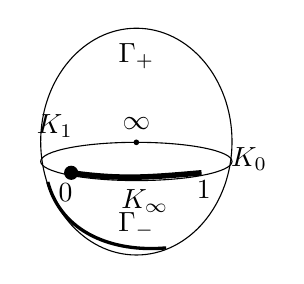
\begin{tikzpicture}[scale=.9]
\draw (0,0) ellipse (1.35 and 1.6);
\draw (0,-.28) ellipse (1.35 and .27);
\draw[line width=2pt] (-.92,-.44) to[out=-8,in=185] (.92,-.44);
\fill (-.92,-.44) circle (.1); \fill (0,-.01) circle (.04);
\node at (-1,-.72) {$0$}; \node at (.95,-.67) {$1$};
\node[above] at (0,.03) {$\infty$};
\node at (0,1.2) {$\Gamma_+$}; \node at (0,-1.18) {$\Gamma_-$};
\node at (-1.15,.22) {$K_1$}; \node at (1.59,-.24) {$K_0$};
\node at (.12,-.84) {$K_\infty$};
\draw[very thick] (-1.25,-.57) to[out=-75,in=185] (.42,-1.5);
\end{tikzpicture}}

joue le rôle de la carte orientée triangulée pondérée universelle, avec $K_0,K_1,K_\infty$ comme arêtes de types $0,1,\infty$ respectivement. Les deux \deleted{faces} \inserted{drapeaux-repères} dans la situation universelle orientée triangulée pondérée sont l'hémisphère nord $\Gamma_+$ et l'hémisphère sud $\Gamma_-$, qui apparaissent comme des ``simplexes'' topologiques, ayant mêmes sommets $0,1,\infty$, et mêmes arêtes $K_0,K_1,K_\infty$ opposées à ceux-ci. Quant aux faces de la situation initiale (21), il y en a une seule, découpe de la sphère $\mathbb P^1(\mathbb C)$ suivant le segment $K_\infty=[0,1]$, avec \deleted{une} \inserted{comme bord l'}\deleted{arête} arête unique $0'(\frac12)_-1'(\frac12)_+0'$ \deleted{qui est} qui est une boucle fermée ayant comme seul sommet $0'\mapsto0$, avec comme ``milieu'' le point $1'\mapsto1$,

\figure{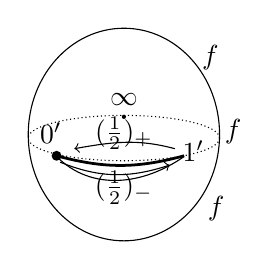
\begin{tikzpicture}[scale=.9]
\draw (0,0) ellipse (1.35 and 1.5);
\draw[densely dotted] (0,-.05) ellipse (1.35 and .32);
\draw[line width=1pt] (-.95,-.3) to[out=-15,in=195] (.85,-.3);
\draw (-.95,-.31) to[out=-45,in=215] (.85,-.31);
\draw[->] (-.9,-.39) to[out=-22,in=198] (.65,-.43);
\draw[->] (.72,-.2) to[out=165,in=10] (-.7,-.2);
\fill (-.95,-.3) circle (.07);
\fill (0,.25) circle (.03);
\node[above] at (0,.27) {$\infty$};
\node at (-1.03,.02) {$0'$};
\node at (.98,-.24) {$1'$};
\node at (0,.02) {$(\frac12)_+$};
\node at (0,-.75) {$(\frac12)_-$};
\node at (1.22,1.08) {$f$}; \node at (1.54,.04) {$f$}; \node at (1.3,-1.04) {$f$};
\end{tikzpicture}}
\margin{L'orientation marquée sur le bord de la découpe est celle induite par l'unique face $f$, avec son orientation habituelle de $\mathbb P^1(\mathbb C)$.}

les deux arcs joignant $0'$ à $1'$ sur le bord de la découpe étant ceux qui passent par $\Gamma_-$ (contenant $(\frac12)_-$) et $\Gamma_+$ (contenant $\unsure{\Gamma_+}$) respectivement. Vu depuis $\infty$, centre de l'unique face, en écartant les deux bords de la découpe, \deleted{\unsure{on en trouve donc cette}}\inserted{celle-ci apparaît} donc comme un disque de centre $\infty$, découpée par les deux rayons \deleted{$(0',\infty)$} $(\infty,0')$ et $(\infty,1')$, joignant $\infty$ à $0\sim0'$ et à $1\sim1'$ respectivement, en les deux repères $\Gamma_+$ et $\Gamma_-$ de la subdivision barycentrique, $\Gamma_+$ ayant \deleted{\unsure{son}} \deleted{\unsure{propre}}\inserted{comme} orientation propre celle induite par $f$, \deleted{\unsure{où}} et $\Gamma_-$ ayant comme orientation propre \uline{l'orientation opposée} de celle induite par $f$. \deleted{\unsure{Une}} \unsure{Par la}

\figure{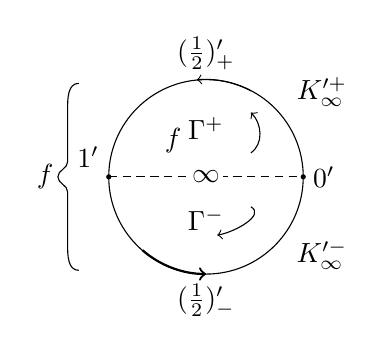
\begin{tikzpicture}[scale=.95]
\draw (0,0) circle (1.3);
\draw[densely dashed] (-1.3,0)--(1.3,0);
\fill (-1.3,0) circle (.035); \fill (1.3,0) circle (.035);
\node[above left] at (-1.3,0) {$1'$}; \node[right] at (1.3,0) {$0'$};
\node[fill=white,inner sep=1pt] at (0,0) {$\infty$};
\node at (0,.65) {$\Gamma^+$}; \node at (0,-.57) {$\Gamma^-$};
\node at (-.44,.48) {\deleted{$f$}};
\draw[->] (.6,.32) to[out=35,in=-45] (.6,.86);
\draw[->] (.6,-.4) to[out=-30,in=10] (.15,-.78);
\draw[->] (.6,1.15) arc (62:95:1.3);
\draw[->,thick] (-.85,-.98) arc (229:270:1.3);
\node[above] at (0,1.3) {$(\frac12)'_+$};
\node[below] at (0,-1.3) {$(\frac12)'_-$};
\node at (1.55,1.13) {$K_\infty^{\prime+}$};
\node at (1.55,-1.05) {$K_\infty^{\prime-}$};
\draw (-1.7,1.25) to[out=180,in=90] (-1.85,.9)--(-1.85,.2)
to[out=-90,in=90] (-1.98,0) to[out=-90,in=90] (-1.85,-.2)--(-1.85,-.9)
to[out=-90,in=180] (-1.7,-1.25);
\node at (-2.15,0) {$f$};
\end{tikzpicture}}
\margin{Attention, si on place $\Gamma^+$ au dessus de l'``équateur'' $0'\infty1'$, $0'$ doit être placé à droite de $\infty$, $1'$ à gauche !}
\margin{62}
